\documentclass[10pt]{exam}
\usepackage[hon]{template-for-exam}
\usepackage{enumitem}
\usepackage{tikz}
\usepackage{multicol}
\usetikzlibrary{shadings,decorations.pathmorphing,arrows.meta}



\def\mytitle{Chapter 6 (Uniform Circular Motion, Gravitation)}
\author{Rohrbach}
\date{\today}

\def\mymaketitle{
  \begin{flushleft}
    {\LARGE \textbf \mytitle \par}
  \end{flushleft}
}


\newcommand{\bs}[2]{\textbf{#1} (\sc #2 Points)}


\begin{document}


\mymaketitle



\newcommand{\stampbox}[1]{

  \hfill
  \begin{tikzpicture}[every text node part/.style={align=center}]
     \node[gray!50,draw,rounded corners] at (0,0) 
      {\sc Stamp \\ \sc Here \\ \small #1 \sc Points};
  \end{tikzpicture}
  \vspace{1em}
  
  \hrule

}

\begin{center}

  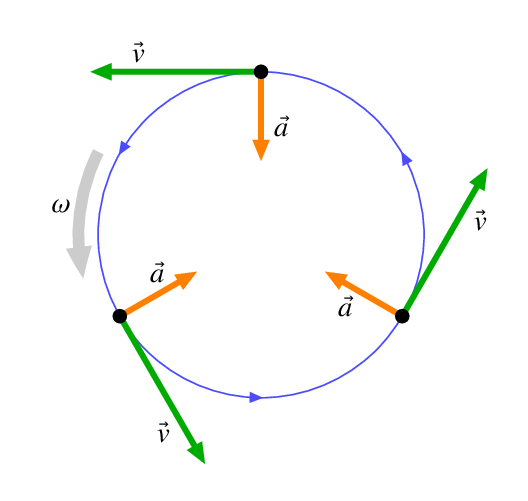
\includegraphics[scale=0.3]{circ.png} \hspace{10em}
  %
  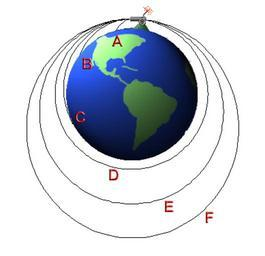
\includegraphics[scale=0.6]{orbitingcannonballs.jpg}
\end{center}

\section*{Homework Check A (collected by XXXXXX)}


%%%%%%%%%%%

\subsection*{Reading}

Please read the following on your own in the OpenStax textbook by the dates given.  It will give good context for class discussion.  Check off when you have completed them.

\vspace{1em}

\begin{checkboxes}
  \choice 6.1 Rotation Angle \& Angular Velocity
  \choice 6.2 Centripetal Acceleration
  \choice 6.3 Centripetal Force
  \choice 6.4 Fictitious Forces
\end{checkboxes}


\subsection*{Problems and Conceptual Question}


Get stamps from your instructor as you complete each of the following problems.  The conceptual questions (CQ) require at least one sentence of explanation.

\vspace{1em}

\noindent
{\sc Stamps will not be given if work is not shown on a separate sheet of paper}

\vspace{1em}


\begin{tabular}{|*{2}{p{7cm}|}}
  \hline
  %
  \bs{Centrip. Force, Acceleration}{5} 
                   & \bs{Multiple Force}{10}  \\ 
                          &               \\[2.5cm]\hline
  %

\end{tabular}


\section*{Equations}


\begin{align*}
  a_C        &= \frac{v^2}{r} &
  \Sigma F_C &= ma_C = \frac{mv^2}{r}  &
  v          &= \frac{2\pi r}{T} 
\end{align*}




%%%%%%%%%%%%%
%%%%%%%%%%%%%

\pagebreak

\mymaketitle

\section*{Homework Check B (collected on Test Day - XXXXX}

\subsection*{Reading}

Please read the following on your own in the OpenStax textbook by the dates given.  It will give good context for class discussion.  Check off when you have completed them.

\vspace{1em}

\begin{checkboxes}
  \choice 6.5 Newton's Law of Universal Gravitation
  \choice 6.6 Satellites \& Kepler's Laws
\end{checkboxes}


\subsection*{Problems and Conceptual Question}


Get stamps from your instructor as you complete each of the following problems.  The conceptual questions (CQ) require at least one sentence of explanation.

\vspace{1em}


\begin{tabular}{|*{2}{p{7cm}|}}
  \hline
  %
  \bs{Friction}{5}       & \bs{Universal Gravitation}{5}  \\
                         & \\[2cm]\hline
  \bs{Satellites}{5}\\  \\[2cm]\cline{1-1}
\end{tabular}



\subsection*{Bonus Problems}

\hfill

\begin{tabular}{|*{4}{p{3.3cm}|}}
  \hline
  %
  P \#10  &  P \#15  &  P \#16  &  P \#17 \\[1.5cm]
  %
  \hline
\end{tabular}

\vspace{1em}
\hrule
\vspace{1em}


\section*{Equations}
\subsection*{New Equations}

\begin{align*}
  a_C        &= \frac{v^2}{r} &
  \Sigma F_C &= ma_C = \frac{mv^2}{r}  &
  v          &= \frac{2\pi r}{T} &
  F_G        &= \frac{Gm_1 m_2}{r^2} \\
  &&&&&& G   &= \SI{6.67e-11}
                {\newton\meter^2\per\kilo\gram^2}
\end{align*}


\subsection*{Old Equations}

\begin{align*}
  \Sigma F &= ma &
  w      &= mg &
  f      &= \mu F_N
\end{align*}


\end{document}